\section{Design Guidelines}
	In order to create the application with a simple to understand and familiar design, design patterns are used in the later prototyping process. The following design patterns are considered useful after a session of brainstorming:
	
	\begin{itemize}
		\item Steps Left Pattern
		\item Cards Pattern
		\item Autocomplete	
		\item Input Feedback Pattern
		\item Rate Content Pattern
		\item Chat Pattern
		\item Product Page Pattern
		\item Gallery Pattern
		\item Calendar Picker Pattern
		\item Password Strength Meter Pattern
		\item Dashboard Pattern
		\item Status-Quo Bias Pattern
		\item Chunking Pattern
		\item Main Navigation
		\item Shortcut Dropdown
		
		% nicht umgesetzt
		\item Preview Pattern
		\item Flagging \& Reporting Pattern
		\item Categorization Pattern
		\item Personalized "My Site"
		\item Pay to Promote Pattern
		\item Reduction Pattern
	\end{itemize}

	\paragraph{Steps Left}
		This pattern is used when both lending and renting parties are communicating via the chat. A overview of already completed and pending steps is displayed next to the chat window.
		
		\begin{figure}[H]
			\centering
			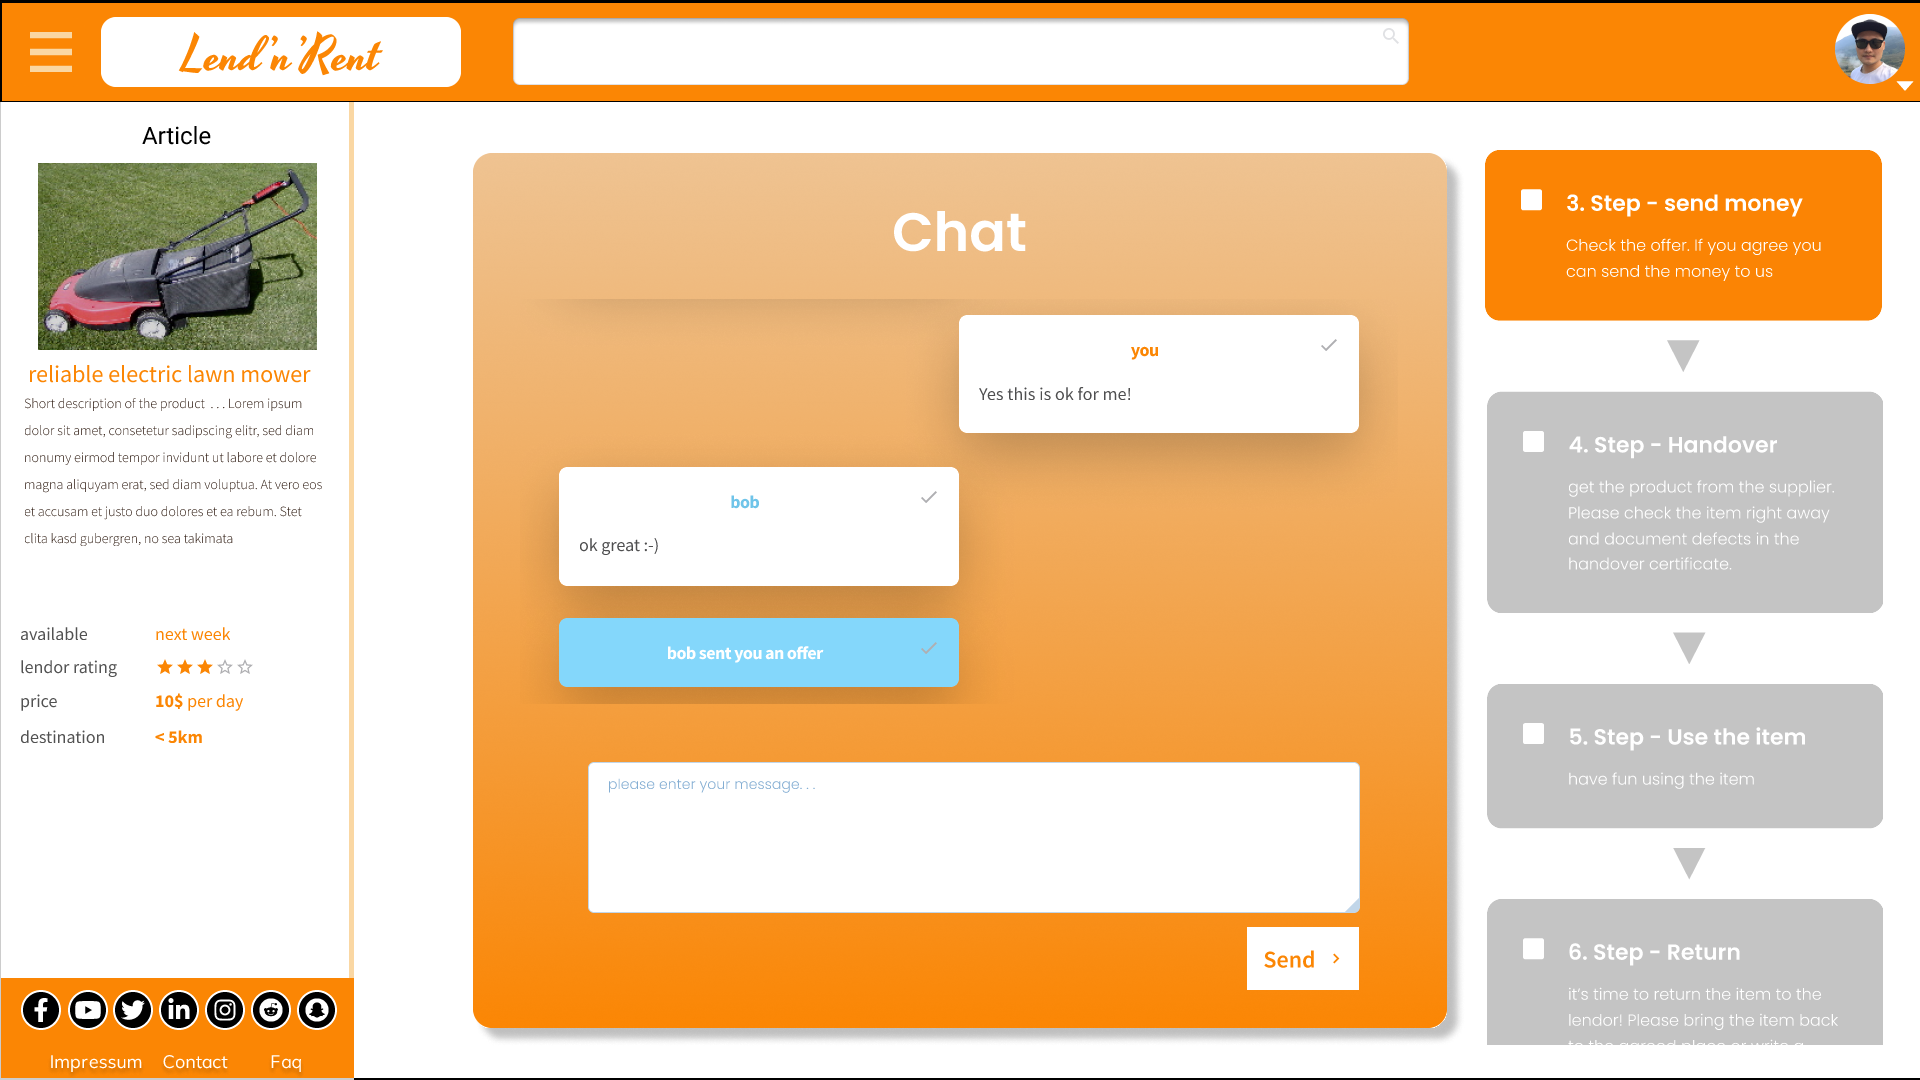
\includegraphics[width=\linewidth]{abb/3_design_guidelines/stepsleft.png}
			\caption{Steps Left pattern next to the chat window}
			\label{fig:stepsleft}
		\end{figure}
	\par
	
	\paragraph{Cards}
		Every offer as well as advertisements in the offer detail page is placed within a separate card including a picture of the item, the description, the price per day, the proximity to the users location and when it is available. With this pattern each offer can be distinguished from the other offers at the first glance.
		
		\begin{figure}[H]
			\centering
			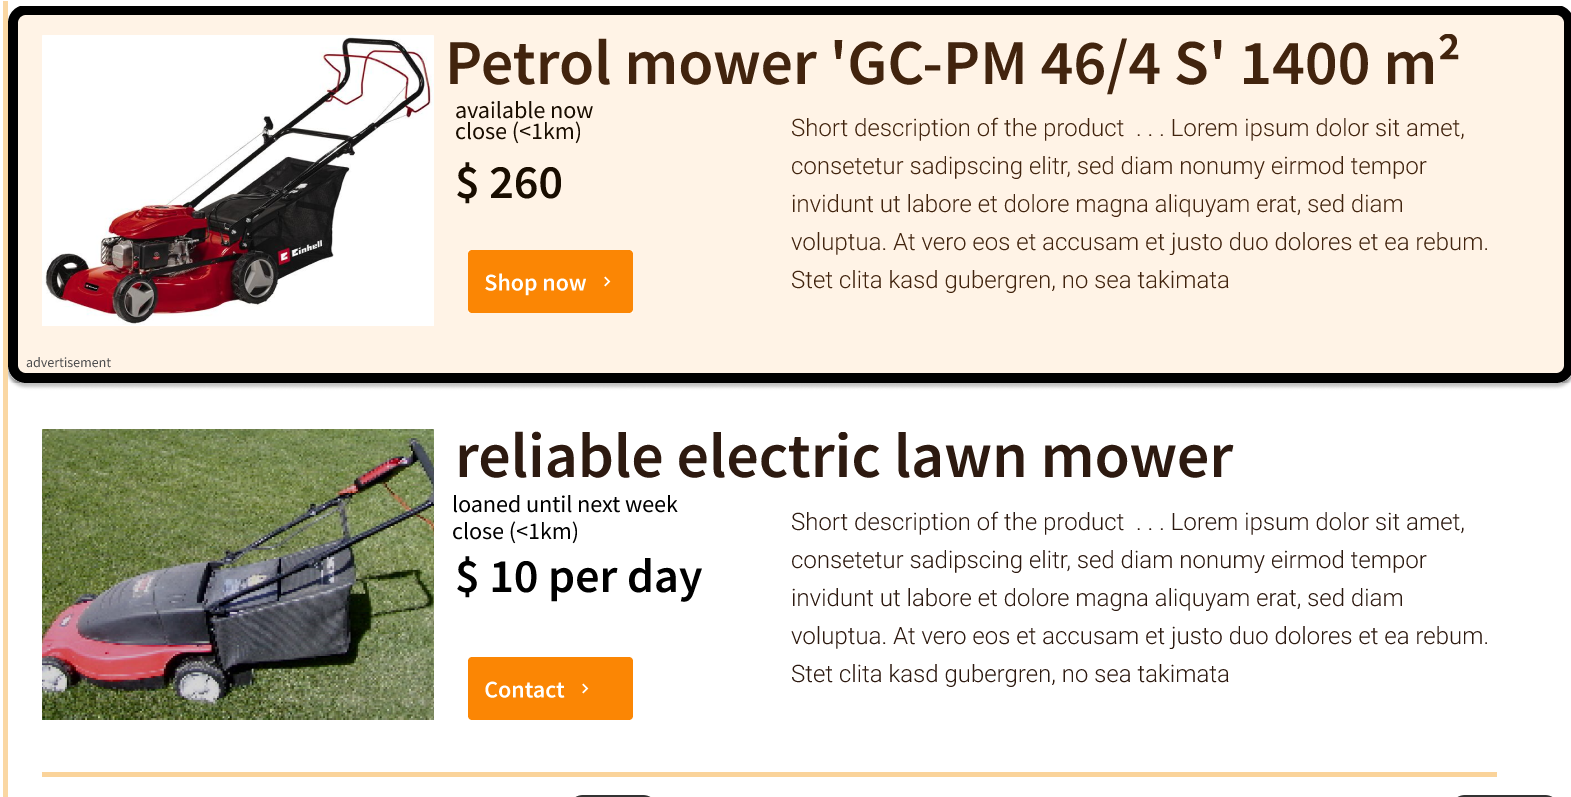
\includegraphics[width=\linewidth]{abb/3_design_guidelines/cards.png}
			\caption{Offer and advertisement cards}
			\label{fig:cards}
		\end{figure}
	\par
	
	\paragraph{Autocomplete and Input Feedback}
		These patterns are used when searching for items and editing the profile. The search query in the search bar and the users address will have suggestions for autocompletion based on previous queries and location services. The inputs will be validated and will have a green tick mark if the format is correct.
	\par
	
	\paragraph{Rate Content}
		When the item is returned after it has been used, both parties can rate each others trustworthiness. This helps future parties to decide if they can trust this user when borrowing from the user or lending to them. This rating takes place in the chat window as a part of the steps to complete the deal.
		
		\begin{figure}[H]
			\centering
			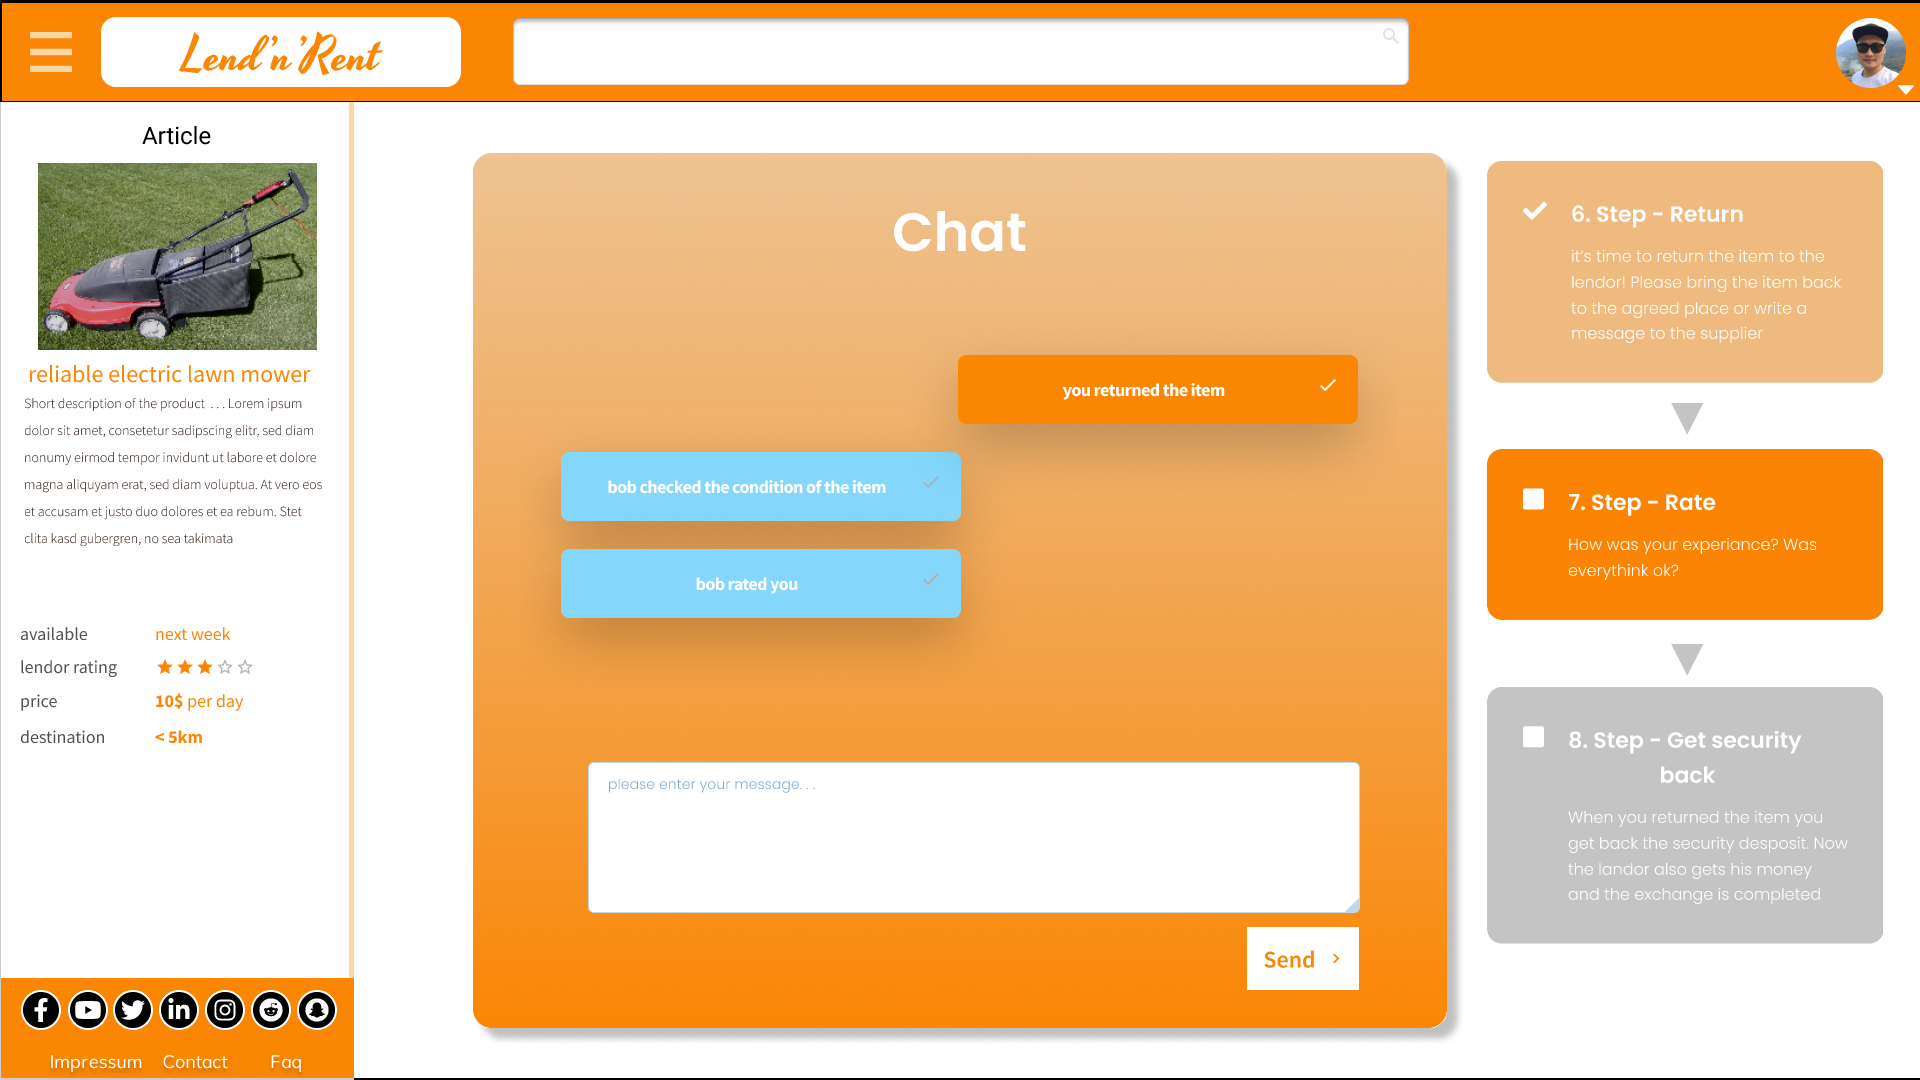
\includegraphics[width=\linewidth]{abb/3_design_guidelines/rate.png}
			\caption{Rating the users}
			\label{fig:rate}
		\end{figure}
	\par
	
	\paragraph{Chat}
		The Chat is the main tool for communication between the lending and renting parties. It is used to 
		\begin{itemize}
			\item contact the lender
			\item agree on the terms of price, deposit and duration
			\item initiate the transfer of money
			\item rate the other party
		\end{itemize}
	\par
	
	\paragraph{Product Page}
		At the product page the user can read the description, contact the lender, see the price, availability and proximity at one glance.
	\par
	
	\paragraph{Gallery}
		Galleries are used on the product detail page when the lender uploads more than one picture for their item. This is used to prevent that all images appear at once and overwhelm the user. It also adds structure to the page.
	\par
	
	\paragraph{Calendar Picker}
		When the lender adds a new offer, they can pick a date to that the item is available for borrowing. The calendar picker appears after clicking the icon next to the input field. This adds comfort for the user because they do not have to enter the date manually and have a visual representation of the weeks.
		
		\begin{figure}[H]
			\centering
			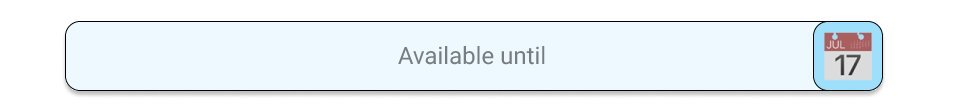
\includegraphics[width=\linewidth]{abb/3_design_guidelines/calendar_picker.png}
			\caption{Calendar picker}
			\label{fig:calendar_picker}
		\end{figure}
	\par
	
	\paragraph{Password Strength Meter}
		When a user creates a new account or changes their current password, the password strength meter will indicated how secure the new chosen password is.
	\par
	
	\paragraph{Dashboard}
		The overview of all messages has certain dashboard functionalities. The user can see all of their incoming and outgoing messages and navigate into the different chat rooms. The incoming and outgoing messages are separated into two tabs.
		\begin{figure}[H]
			\centering
			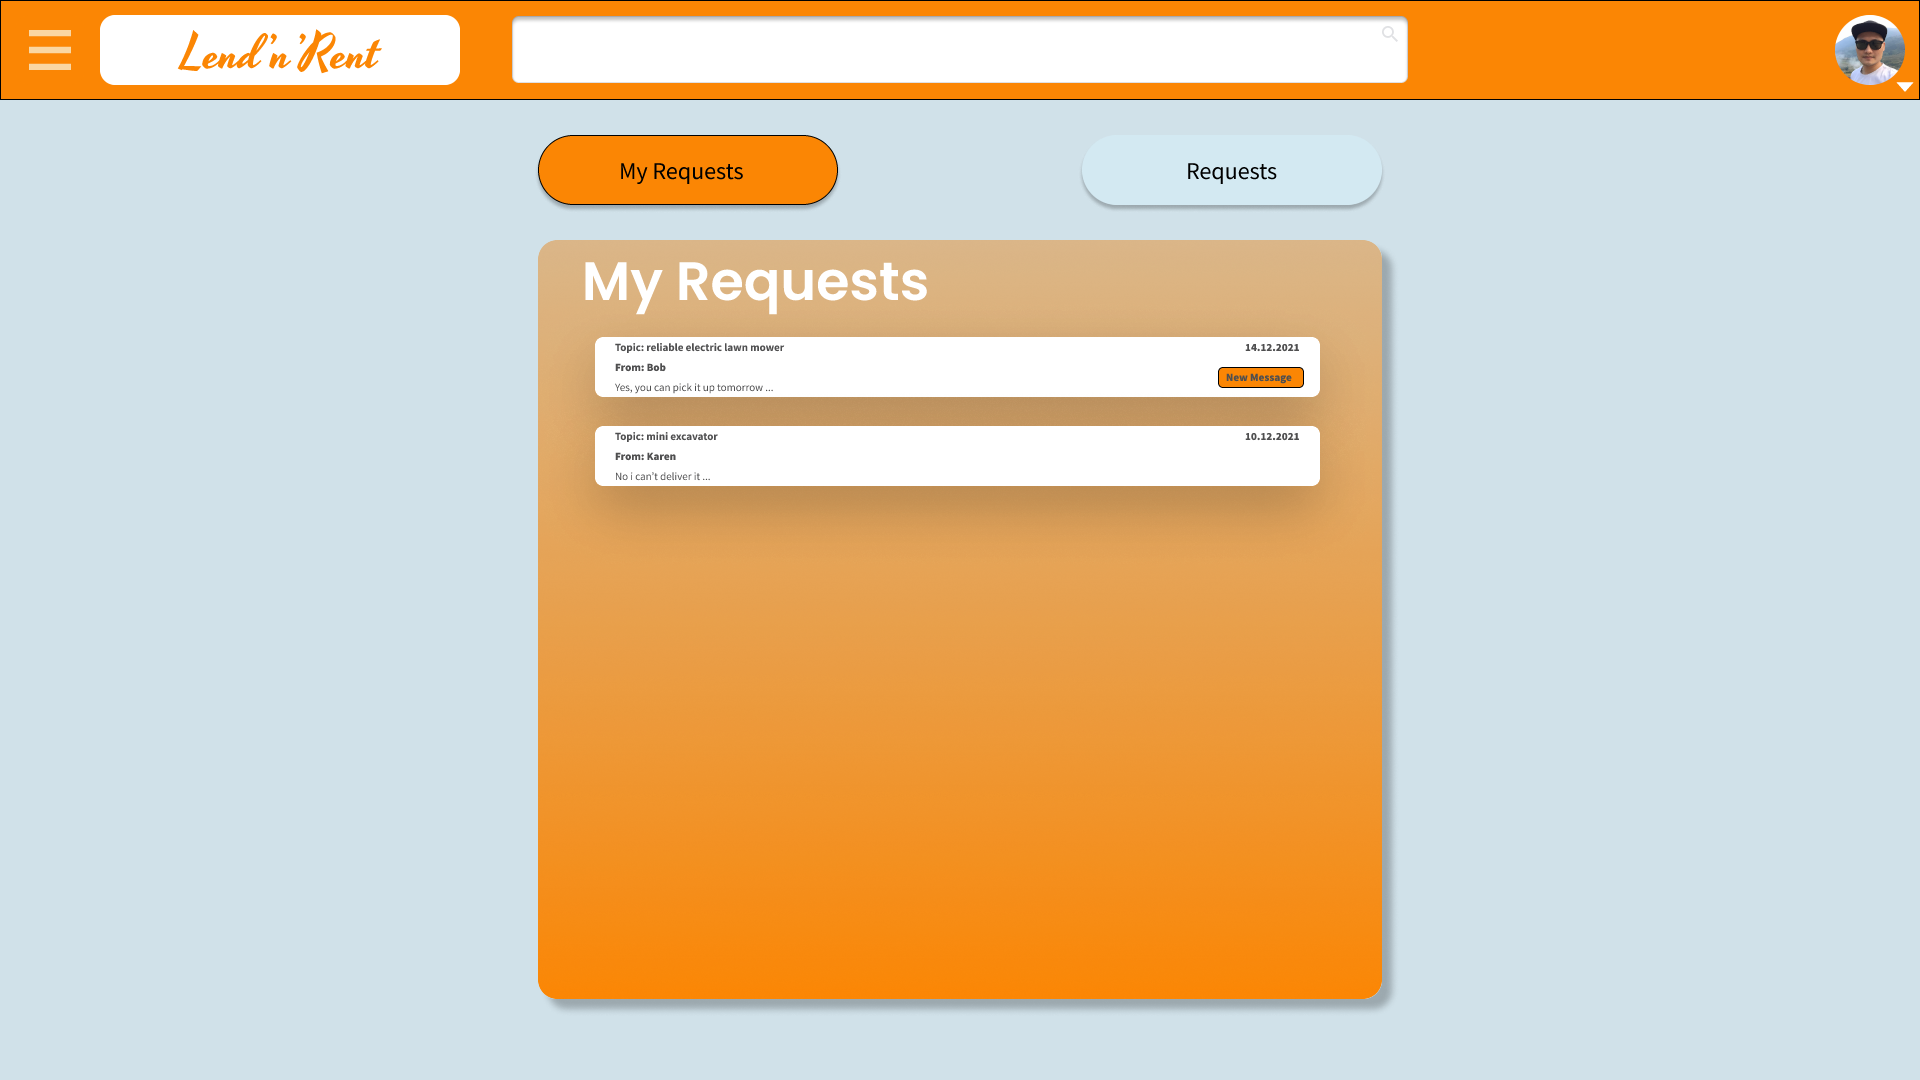
\includegraphics[width=0.49\linewidth]{abb/3_design_guidelines/messages_1.png}
			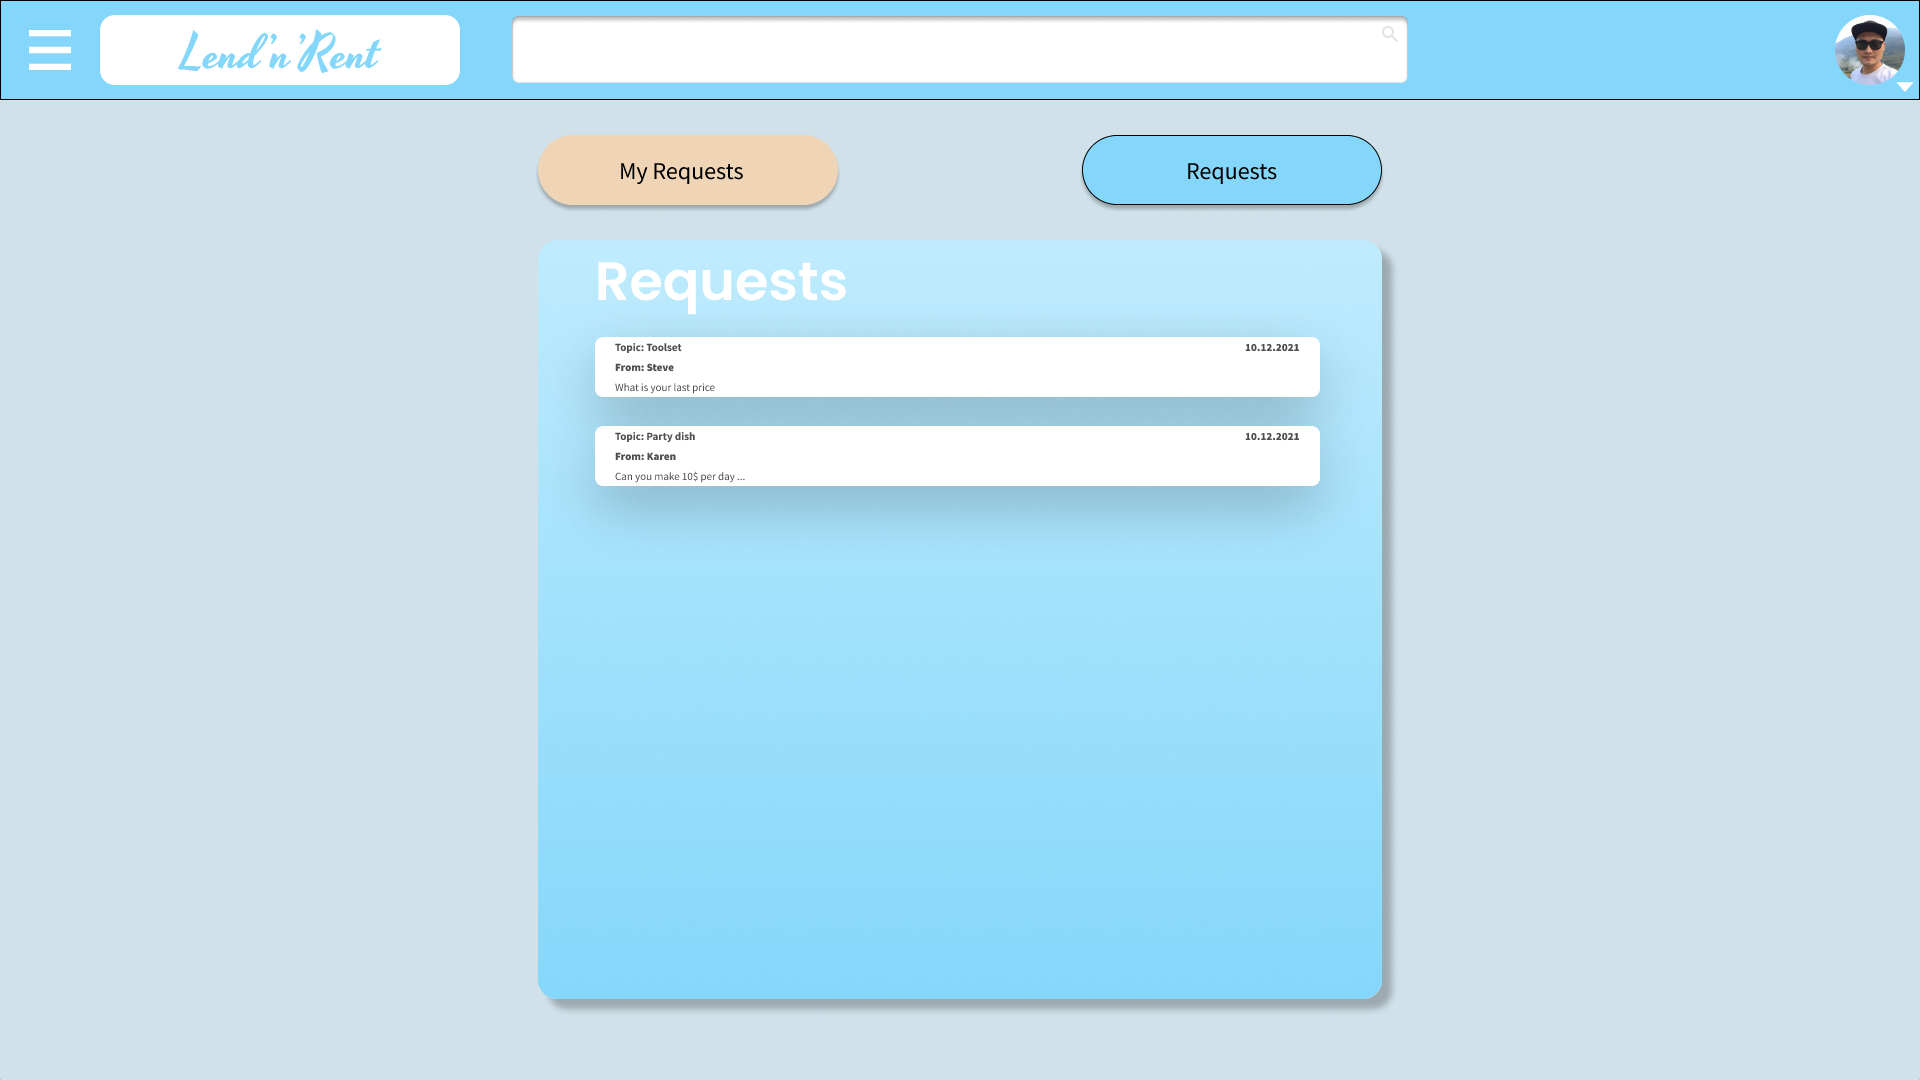
\includegraphics[width=0.49\linewidth]{abb/3_design_guidelines/messages_2.png}
			\caption{Message dashboard}
			\label{fig:message_dashboard}
		\end{figure}
	\par
	
	\paragraph{Status-Quo Bias}
		The landing pages color scheme is set to orange that signals the user that they are using the borrowing part of the platform. This decision was made because most of the time the users probably want to search for items and compare them with their needs. The assumption that was made is that only more experienced users want to offer their items for borrowing.
	\par
	
	\paragraph{Shortcut Dropdown}
		The user can filter their search results by category either by navigating through a tree of submenus or by using a dropdown menu above the search results.
		\begin{figure}[H]
			\centering
			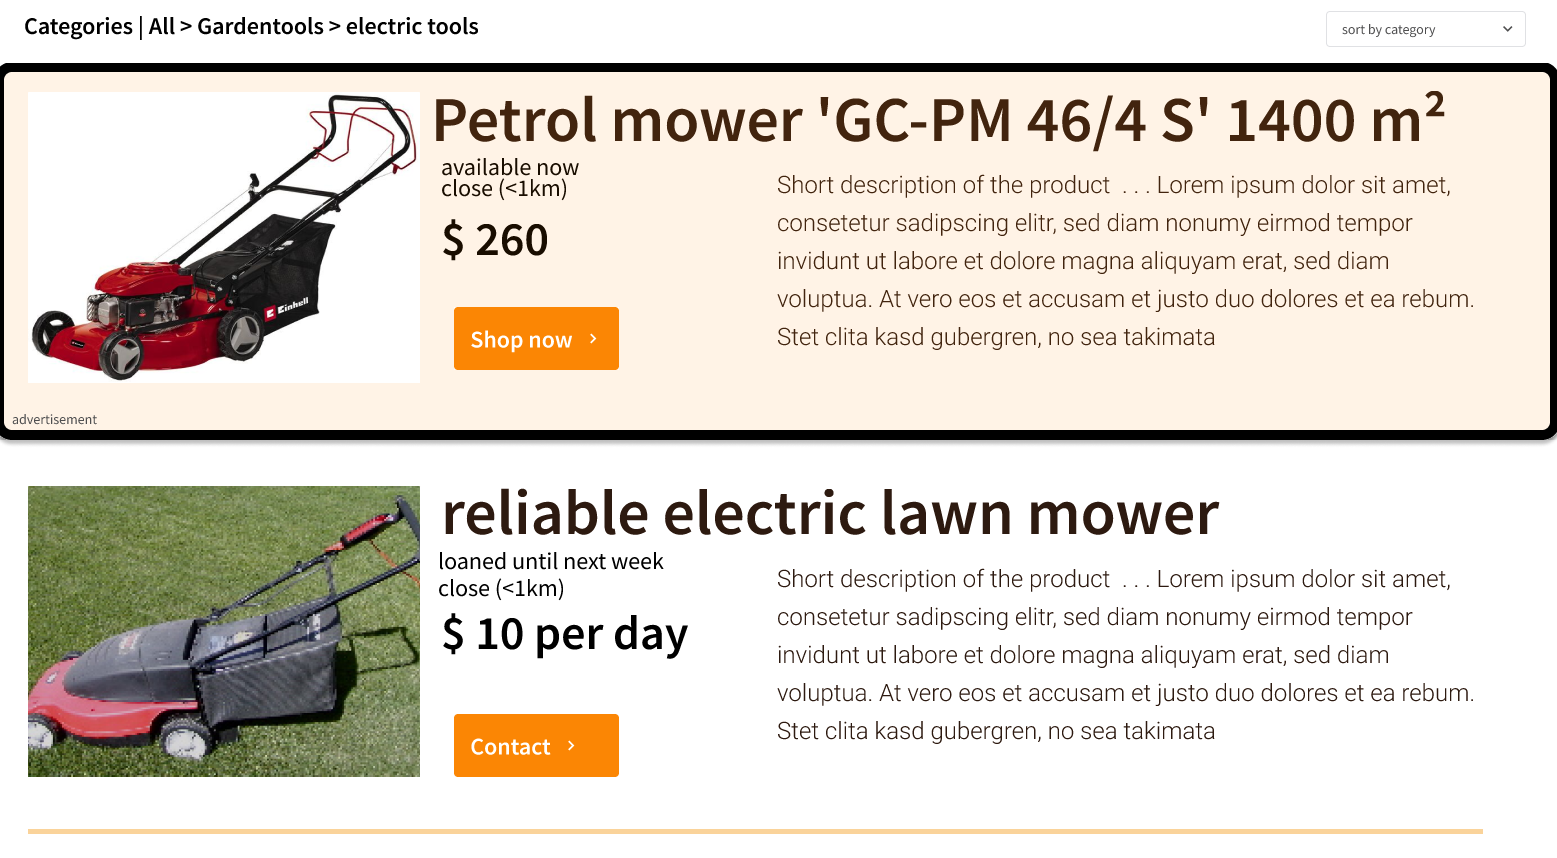
\includegraphics[width=\linewidth]{abb/3_design_guidelines/dropdown_shortcut.png}
			\caption{Dropdown Shortcut}
			\label{fig:dropdown_shortcut}
		\end{figure}
	\par
	
	
	
	